\documentclass[10pt,a4paper]{article}

\usepackage{appendix}
\usepackage{graphicx}
\usepackage{parskip}
\usepackage{listings}
\usepackage{caption}
\usepackage{subcaption}
\usepackage{amsmath}
\usepackage{listings}
\usepackage{xcolor}
\usepackage[most]{tcolorbox}

%%%%%%%%%%%%%%%%%%%%%%%%%%%%%%%%%%%%%%%%%%%%%%%%%%%%%%%%%%%%%%%%%%%%%%%%%%%%%%%%%%%%%%%%%%%%%%%%%%%%%%%%%%
\definecolor{codegreen}{rgb}{0,0.6,0}
\definecolor{codegray}{rgb}{0.5,0.5,0.5}
\definecolor{codepurple}{rgb}{0.58,0,0.82}
\definecolor{backcolour}{rgb}{1,1,1}

\lstdefinestyle{mystyle}
{
    backgroundcolor=\color{backcolour},   
    commentstyle=\color{codegreen},
    keywordstyle=\color{magenta},
    numberstyle=\tiny\color{codegray},
    stringstyle=\color{codepurple},
    basicstyle=\ttfamily\footnotesize,
    breakatwhitespace=false,         
    breaklines=true,                 
    captionpos=b,                    
    keepspaces=true,                 
    numbers=left,                    
    numbersep=5pt,                  
    showspaces=false,                
    showstringspaces=false,
    showtabs=false,                  
    tabsize=2
}

\lstset{style=mystyle}
%%%%%%%%%%%%%%%%%%%%%%%%%%%%%%%%%%%%%%%%%%%%%%%%%%%%%%%%%%%%%%%%%%%%%%%%%%%%%%%%%%%%%%%%%%%%%%%%%%%%%%%%%%

\lstset{basicstyle=\ttfamily, breaklines = true, tabsize=2}
\graphicspath{ {./Images/} }
\setlength{\parskip}{1em}
\begin{document}
%%%%%%%%%%%%%%%%%%%%%%%%%%%%%%%%%%%%%%%%%%%%%%%%%%%%%%%%%%%%%%%%%%%%%%%%%%%%%%%%%%%%%%%%%%%%%%%%%%%%%%%%%%

\begin{titlepage}
	\centering
	{\scshape\LARGE Imperial College London \par}
	\vspace{1cm}
    {\scshape\Large ISA and Compilers: Year 2\par}
    \vspace{1.5cm}
	{\huge\bfseries Processor: Control and Data Path \par}
	\vspace{2cm}
	{\Large\ Xin Wang }
	\vfill
	{\large \today\par}
\end{titlepage}

%%%%%%%%%%%%%%%%%%%%%%%%%%%%%%%%%%%%%%%%%%%%%%%%%%%%%%%%%%%%%%%%%%%%%%%%%%%%%%%%%%%%%%%%%%%%%%%%%%%%%%%%%%

\begin{abstract}
    Chapter 1 explains that the performance of a computer is determined by three key factors: 
    Instruction count, Clock cycle time and Clock cycles per instruction (CPI).

    Chapter 2 explains that the compiler and the instruction set architecture determine the
    instruction count required for a given program. However most importantly, the implementation 
    of the processor determines both the clock cycle time and the number of clock cycles per
    instruction. In this chapter, the datapath and control unit for two different implementations of
    the MIPS instruction set are constructed.

    This chapter starts an explanation of the principles and techniques used in implementing a
    processor, starting with an abstract and simplified overview. It is followed by a section that
    builds up a datapath and constructs a simple version of a processor sufficient to implement an
    instruction set like MIPS. 
    
    The bulk of the chapter covers a realistic pipelined MIPS implementation that develops the
    concepts necessary to implement more complex instruction sets, like the x86.
\end{abstract}

%%%%%%%%%%%%%%%%%%%%%%%%%%%%%%%%%%%%%%%%%%%%%%%%%%%%%%%%%%%%%%%%%%%%%%%%%%%%%%%%%%%%%%%%%%%%%%%%%%%%%%%%%%

\tableofcontents
\pagebreak

%%%%%%%%%%%%%%%%%%%%%%%%%%%%%%%%%%%%%%%%%%%%%%%%%%%%%%%%%%%%%%%%%%%%%%%%%%%%%%%%%%%%%%%%%%%%%%%%%%%%%%%%%%
\section{The basic MIPS implementation}

From Year 1 DECA, the following concepts are already covered:
\begin{itemize}
    \item How to split instruction into opcode and operands.
    \item How to encode instructions as bits.
    \item How to build an ALU.
\end{itemize}

This chapter focuses on how to build a datapath and design a suitable control path. To aid in this
process, an implementation that including a subset of the core MIPS instruction set:
\begin{itemize}
    \item \textbf{Memory-access instructions}: load word (\texttt{lw}) and store word (\texttt{sw})
    \item  \textbf{Register-based instructions}: \texttt{add}, \texttt{sub}, \texttt{AND},
    \texttt{OR}, and \texttt{slt}
    \item \textbf{Branch instructions}: branch equal (\texttt{beq}) and jump (\texttt{j})
\end{itemize}
is examined. These instructions illustrates the key principles used in creating a datapath and designing 
the control. The implementation of the remaining instructions is similar.

The importance of this chapter is to notice how the instruction set architecture determines many aspects of the implementation, and how the choice of various implementation strategies affects the clock rate and CPI 
for the computer.  Many of the key design principles introduced in earlier can be illustrated by
looking at the implementation.

%%%%%%%%%%%%%%%%%%%%%%%%%%%%%%%%%%%%%%%%%%%%%%%%%%%%%%%%%%%%%%%%%%%%%%%%%%%%%%%%%%%%%%%%%%%%%%%%%%%%%%%%%%
\subsection{Implementation overview}

Much of the implementations of these instructions is the same, independent of the exact class of the
instruction. For every instruction, the first two steps are identical:
\begin{enumerate}
    \item Send the Program Counter (PC) content to the Memory which contains the code and 
    fetches the instruction from the Memory.
    \item Read one or two registers, using fields of the instruction to select which of the
    registers to read e.g. for the \texttt{lw} instruction, only one register is read, but other
    instructions like \texttt{add} would require reading two registers.
\end{enumerate}

After these two steps, the actions required to complete the instruction depend on the instruction
classes. For each of the three instruction classes the actions are largely the same - independent of
the exact instruction. The simplistic and regularity of the MIPS instruction set results in making
the execution of many of the instruction classes similar.

A high-level view of a MIPS implementation is given, emphasising on the \textbf{various functional
units}  and \textbf{interconnection fo function units}. 
\begin{figure} [h!]
    \centering
    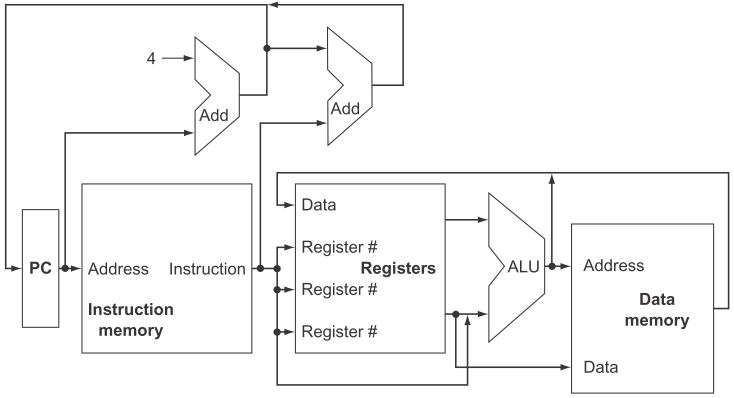
\includegraphics[scale=0.7]{High level MIPS view.JPG}
    \caption{A high-level view of a MIPS implementation}
\end{figure}

Data process:
\begin{enumerate}
    \item All instructions start with using the \textit{PC} to supply the \textbf{instruction
    address} to the \textit{Memory} containing instructions and data.
    \item After the instruction is fetched, the fields of that instruction is processed and
    determines the register operands to be used.
    \item Required register operands are fetched from Memory.
    \item  Once the register operands are fetched, it is operated on differently by the ALU:
    \begin{itemize}
        \item To compute a memory address (for a load or store)
        
        The ALU result is used as an address to either store a value from the registers or load a value from memory into the registers.
        \item To compute an arithmetic result (for an integer arithmetic-logical instruction)
        
        The result from the ALU must be written to a register.
        \item To compare (for a branch)
        
        Branches require the use of the ALU output to determine the next instruction 
        address, which comes either from the ALU (where the PC and branch off set are summed) or from an adder that increments the current PC by 4.
    \end{itemize}
\end{enumerate}

This view shows most of the flow of data through the processor but it omits two important aspects of
instruction execution:
\begin{enumerate}
    \item Note in several places, the diagram shows data going into a particular unit as coming from
    two different sources merging into one e.g. the data coming into the \textit{PC} is a merger
    from the two \textit{Add} blocks.

    Practically, these data lines are not wired together. A logic element is added that chooses from 
    the multiple sources and selects one source only based on the setting of its control lines. This
    logic element is called a \textbf{multiplexor} or \textbf{data selector}.
    \item Several of the units must be controlled depending on the type of instruction e.g. data
    memory must read on a load and written on a store. Register files must be written only on
    a load or an arithmetic-logical instruction. Control lines that are set depending on the basis
    of the various fields in the instruction control these operations.
\end{enumerate}

The final overview diagram shows the datapath of the previous with the three required multiplexors added
and the control lines for the major functional units.
\begin{figure} [h!]
    \centering
    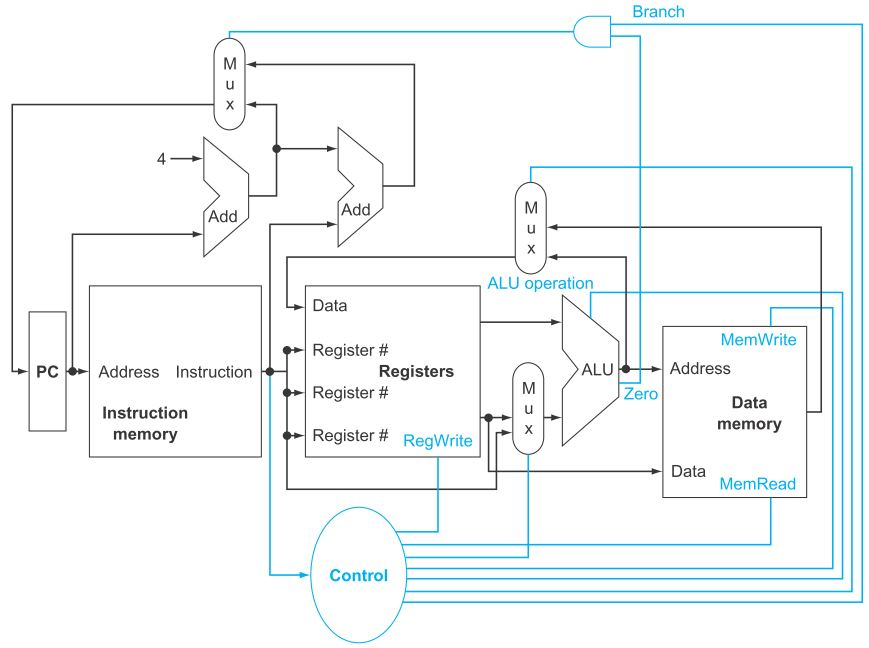
\includegraphics[scale=0.65]{Data path}
    \caption{Implementation of MIPS subset including necessary multiplexors and control lines. }
\end{figure} 
\begin{enumerate}
    \item \textbf{Control Unit} has the \textit{instruction} as an input and controls the \textit{control lines} for the functional units and two of the multiplexors. 
    \item \textbf{Top multiplexor} chooses between whether $PC + 4$ or the branch destination
    address based on the Zero output of the \textit{ALU} i.e. performs the comparison of a \texttt{beq}
    instruction.
    \item  \textbf{Middle multiplexor} used to steer the output of the \textit{ALU} (in the case of
    an arithmetic-logical instruction) or the \textit{data memory} (in the case of a load) into the
    register file.
    \item  \textbf{Bottom multiplexor} used to determine if the second \textit{ALU} input is from
    the \textit{registers} (for an arithmetic-logical instruction or a branch) or from the
    \textit{offset field of the instruction} (for a load or store). 
\end{enumerate}

The regularity and simplicity of the MIPS instruction set allows a simple decoding process to be
used to determine how to set the control lines.

%%%%%%%%%%%%%%%%%%%%%%%%%%%%%%%%%%%%%%%%%%%%%%%%%%%%%%%%%%%%%%%%%%%%%%%%%%%%%%%%%%%%%%%%%%%%%%%%%%%%%%%%%%
\section{Logic design conventions}

When implementing the hardware logic of a computer, how it operates and how the computer is clocked
are important aspects to consider.

\begin{tcolorbox}[breakable,colback=white]
\textbf{Combinational}: The output of the element only depends on the current inputs. Common
combinational elements are AND gate or ALU.
\\
\\
\textbf{State element}:  An element some internal storage i.e. a memory element. Common state
elements are flip-flops, registers and memory.
\end{tcolorbox}

The datapath in MIPS consist of two different types of logic elements: 
\begin{itemize}
    \item Elements that operate on data values:
    
    The elements are all \textbf{combinational}. Given the same input, a combinational element
    always produces the same output because it has no internal storage.

    \item Elements that contain \textbf{state}:
    
    State elements are important elements as it characterises the computer. A state element has
    \textbf{at least two inputs}:  
    \begin{enumerate}
        \item The data value to be written into the element
        \item The clock that determines when the data value can be written. A state element can be read at any time.
    \end{enumerate}
    and one output that provides the value that \textbf{was written in an earlier clock cycle}.
\end{itemize}

The opposite of \textbf{combinational} is \textbf{sequential}. Logic components that contain state
are sequential since the outputs depend on both \textbf{its inputs} and \textbf{the contents of the
internal state}.

%%%%%%%%%%%%%%%%%%%%%%%%%%%%%%%%%%%%%%%%%%%%%%%%%%%%%%%%%%%%%%%%%%%%%%%%%%%%%%%%%%%%%%%%%%%%%%%%%%%%%%%%%%
\subsection{Clocking}

\begin{tcolorbox}[breakable,colback=white]
\textbf{Clocking methodology}: The approach used to determine when data is valid and stable relative
to the clock.
\end{tcolorbox}

A clocking methodology is required to make hardware predictable by specifying the timing of reads
and writes. It prevents the situation where reading and writing occurs simultaneously. This would
result ina  glitch - unpredictable behaviour. 

The easiest of clocking methodology is \textbf{edge-triggered methodology}. There are two types:
\textbf{positive-edge triggered} and \textbf{negative-edge triggered}.
\begin{tcolorbox}[breakable,colback=white]
\textbf{Edge-triggered clocking:} A clocking scheme in which all state changes occur on a clock
edge. Any values stored in a sequential logic element are updated only on a clock edge
\end{tcolorbox}

The inputs are values that were written in a previous clock cycle, while the outputs are values 
that can be used in a following clock cycle.
\begin{figure} [h!]
    \centering
    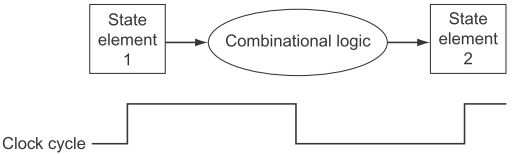
\includegraphics[scale=0.6]{Clocking.JPG}
    \caption{Relation between combinational logic, state elements and the clock.}
\end{figure}

\textbf{Single clock cycle} - Time taken for all signals to propagate from state element 1, through the combinational logic, and to state element 2.

\begin{tcolorbox}[breakable,colback=white]
\textbf{Control signal}: A signal used for multiplexor selection or for directing the operation of a
functional unit.
\\
\\
\textbf{Data signal}: A signal that contains information that is operated on by a functional unit.
\end{tcolorbox}

A state element is either written on \textbf{every clock edge} or controlled by \textbf{an explicit
control signal}. The state element is changed \textbf{only when the write control signal is asserted
and a clock edge occurs}.

%%%%%%%%%%%%%%%%%%%%%%%%%%%%%%%%%%%%%%%%%%%%%%%%%%%%%%%%%%%%%%%%%%%%%%%%%%%%%%%%%%%%%%%%%%%%%%%%%%%%%%%%%%
\section{Building the Data Path}

\begin{tcolorbox}[breakable,colback=white]
\textbf{Datapath element}: A unit used to operate on or hold data within a processor. In the MIPS
implementation, the datapath elements include the instruction and data memories, the register file, the ALU, and adders.
\end{tcolorbox}

The three-stage compositional approach: 
\begin{enumerate}
    \item Create each datapath independently by examining the major components required to execute
    each class of MIPS instructions.
    \item Combine datapaths, sharing whenever possible.
    \item Add control to dynamically select the correct datapaths depending on the instructions.
    \begin{itemize}
        \item Data-independent: i.e. add and load
        \item Data-dependent: i.e. branches
    \end{itemize}
\end{enumerate}

The fundamental components of any processor design is the following:
\begin{enumerate}
    \item PC: Fetch the instruction from memory.
    \item Memory: Contains data and instructions.
    \item Adder: To form the ALU. 
\end{enumerate}
\begin{figure} [h!]
    \centering
    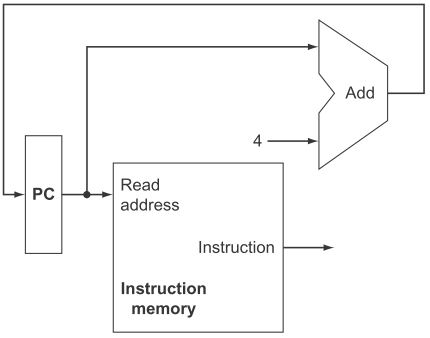
\includegraphics[scale=0.6]{Core data path.JPG}
    \caption{The core portion of the datapath for fetching instructions and incrementing PC.}
\end{figure}

%%%%%%%%%%%%%%%%%%%%%%%%%%%%%%%%%%%%%%%%%%%%%%%%%%%%%%%%%%%%%%%%%%%%%%%%%%%%%%%%%%%%%%%%%%%%%%%%%%%%%%%%%%
\subsection{Register (R)-based instructions}

R-type or arithmetic-logical instructions e.g. \texttt{add}, \texttt{sub}, \texttt{AND} and
\texttt{slt}. The instructions \textbf{read} two registers, \textbf{perform} an ALU operation on the
contents of the registers, and \textbf{write} the result to a register.

\begin{tcolorbox}[breakable,colback=white]
    \textbf{Register file}: A state element that consists of a set of registers that can be read and
    written by supplying a register number to be accessed. The processor’s 32 general-purpose
    registers are stored in it. 
\end{tcolorbox}

\begin{figure} [h!]
    \centering
    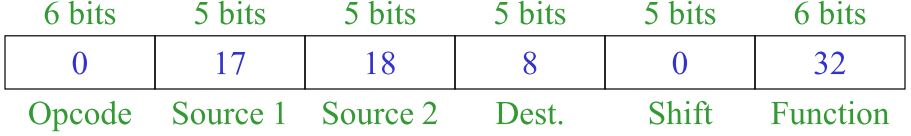
\includegraphics[scale=0.5]{R type.JPG}
\end{figure}

Three register operands: Read two data words from the register file and write one data
word into the register file \textbf{for each instruction}.
    \begin{itemize}
        \item For each data word to be read from the registers: $1)$ an input to \textit{register file}
        specifying the \textit{register number} to be read, $2)$ an output from the \textit{register
        file} that will carry the value read from the \textit{registers}.
        \item Writing a data word, two inputs needed: $1)$ Specify the register number to be 
        written to, $2)$ Supply the data to be written into the register. 

        Process is controlled by the write control signal, which must be asserted for a write to occur at the clock edge. 
    \end{itemize}

\begin{figure} [h!]
    \centering
    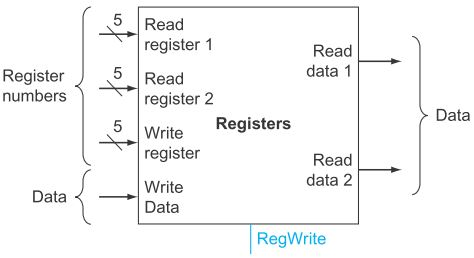
\includegraphics[scale=0.7]{Register file.JPG}
    \caption{Register file: The inputs carrying the register number to the register file are all $5$ bits wide, whereas the lines carrying data values are $32$ bits wide.}
\end{figure}

\textbf{Example 1}: \texttt{add \$5, \$6, \$7 \#reg[5] = reg[6] + reg[7]}
\begin{figure} [h!]
    \centering
    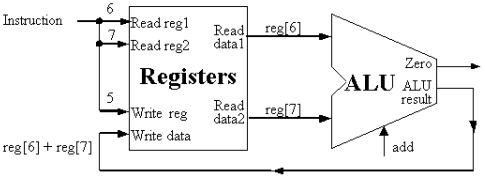
\includegraphics[scale=0.8]{R type example.JPG}
    \caption{Data path flow of R type instructions}
\end{figure}

\pagebreak
%%%%%%%%%%%%%%%%%%%%%%%%%%%%%%%%%%%%%%%%%%%%%%%%%%%%%%%%%%%%%%%%%%%%%%%%%%%%%%%%%%%%%%%%%%%%%%%%%%%%%%%%%%
\subsection{Memory access (I) type instructions}

\begin{figure} [h!]
    \centering
    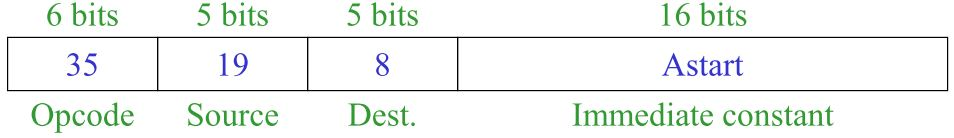
\includegraphics[scale=0.5]{I type.JPG}
\end{figure}

These instructions compute a memory address by adding the base register \texttt{\$t2}, to the 16-bit
signed off-set field contained in the instruction \texttt{\$t1}. Consider the MIPS instructions:
\begin{itemize}
    \item \textit{load} word instruction: \texttt{lw \$t1, offset\_value(\$t2)}
    
    Value read from memory must be \textbf{written into} the \textit{register file} in the specified register \texttt{\$t1}.
    \item \textit{store} word instruction: \texttt{sw \$t1, offset\_value(\$t2)}
    
    Value to be stored must also be \textbf{read from} the \textit{register file} where it resides in \texttt{\$t1}.
\end{itemize}

This type of instructions will require the following components:
\begin{itemize}
    \item \textit{ALU}: Calculate the offset address value.
    \item \textit{Memory}: Store data and instruction.
    \item \textit{Sign extend}: Extend the 16-bit off-set field \textbf{of the instruction} to a
    32-bit signed value to be added on by the \textit{ALU}.
\end{itemize}

\textbf{Example 1}: \texttt{lw \$5, offset(\$6) \#reg[5] = M[reg[6] + offset] }
\begin{figure} [h!]
    \centering
    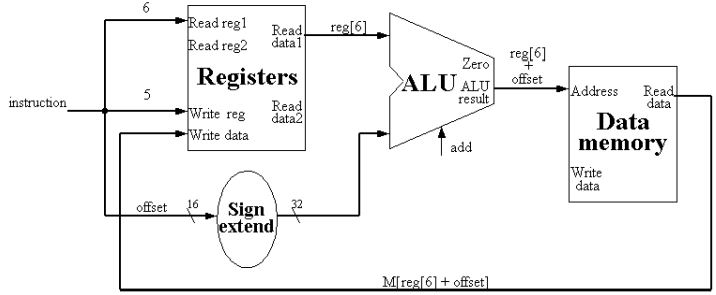
\includegraphics[scale=0.8]{I type example 1.JPG}
    \caption{Data path flow of I type instruction \texttt{lw}}
\end{figure}

\pagebreak
\textbf{Example 2}: \texttt{sw \$5, offset(\$6) \# M[reg[6] + offset] = reg[5]}
\begin{figure} [h!]
    \centering
    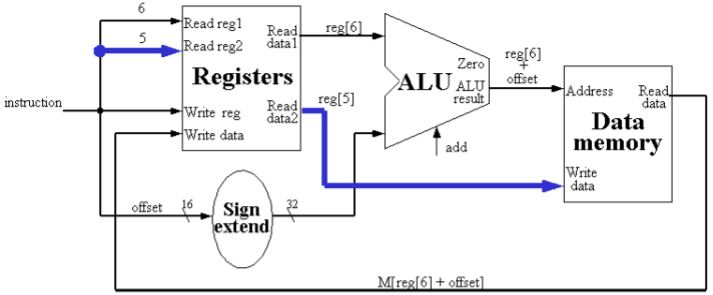
\includegraphics[scale=0.8]{I type example 2.JPG}
    \caption{Data path flow of I type instruction \texttt{rw}}
\end{figure}

Branch instructions \texttt{beq} are part of I-type instructions.
\begin{lstlisting}[numbers=none]
    beq  $t1,$t2,offset.
\end{lstlisting}
The \texttt{beq} instruction has three operands: 
\begin{itemize}
    \item Two registers that are used for comparing for equality.
    \item A 16-bit off-set used to compute the \textbf{branch target address} relative to the branch
    instruction address.
\end{itemize}

\begin{tcolorbox}[breakable,colback=white]
    \textbf{branch target address} = The address specified in a branch, which becomes the new
    \textit{PC} value if the branch is taken. In the MIPS architecture the branch target is given by: 
    \begin{itemize}
        \item Sum of the off-set field of the instruction
        \item Address of the instruction following the branch
    \end{itemize}
\end{tcolorbox}

To implement this instruction, the branch target address must be computed by adding the
\textbf{sign-extended off-set field} of the instruction to the \textit{PC}. There are two important
aspects to remember about the MIPS architecture:
\begin{enumerate}
    \item  The MIPS instruction set architecture requires that the \textbf{base address used in the
    branch address calculation} is the \textbf{address of the instruction following the branch}.

    Remember the address of the next instruction is simply \texttt{PC + 4}, so it is easy to use
    this value as the base for computing the branch target address.
    
    \item  The MIPS architecture also states that \textbf{the off-set field is shifted left $2$ bits} i.e. it is \textbf{a word off-set}. This shift increases the effective range of the off-set field by a
    factor of $4$.

    To deal with that complication, we will need to shift the off-set field by $2$.
\end{enumerate} 

As well as computing the branch target address, the processor must determine whether the next
instruction is:
\begin{itemize}
    \item The instruction that follows sequentially:
    
    If the operands are not equal i.e. conditions are not true, the incremented \texttt{PC} value
    will replace the current \texttt{PC} value as normal.

    \item The instruction at the branch target address: 
    
    The operands are equal i.e. conditions is true, the branch target address becomes the new
    \texttt{PC} value.
\end{itemize}

SO in summary the branch datapath must do \textbf{two operations}: 
\begin{itemize}
    \item Compute the branch target address.
    \item Compare the register contents.
\end{itemize} 

Note: Branches affect the \textbf{instruction Fetch portion} of the datapath.
\begin{figure} [h!]
    \centering
    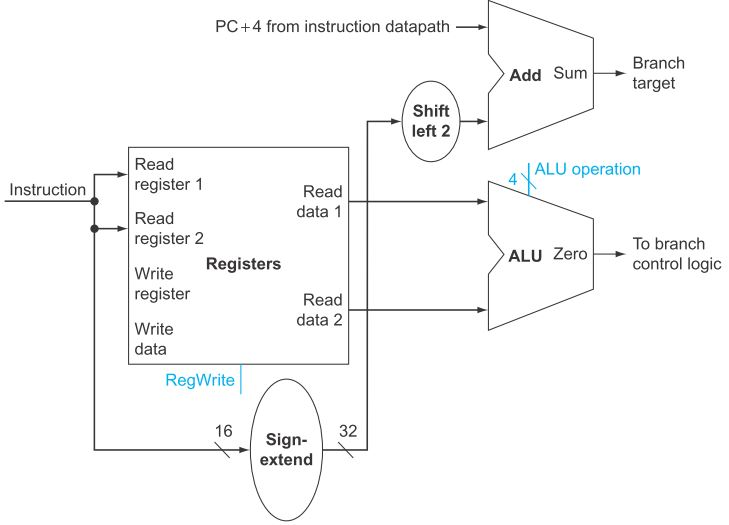
\includegraphics[scale=0.7]{Branch.JPG}
    \caption{Datapath for a branch using the \texttt{ALU} to evaluate the branch condition and 
    a separate adder \texttt{Add} to compute the branch target as the sum of the incremented
    \texttt{PC} and the \textbf{sign-extended, lower 16 bits} of the instruction, shifted left 2
    bits. The control logic from the \texttt{ALU} is used to decide whether the incremented PC or branch target should replace the PC.}
\end{figure} 

\pagebreak
%%%%%%%%%%%%%%%%%%%%%%%%%%%%%%%%%%%%%%%%%%%%%%%%%%%%%%%%%%%%%%%%%%%%%%%%%%%%%%%%%%%%%%%%%%%%%%%%%%%%%%%%%%
\subsection{Combining into single data path}

Now a simple datapath for the core MIPS architecture is formed by adding the two datapath designs. \par
\begin{figure} [h!]
    \centering
    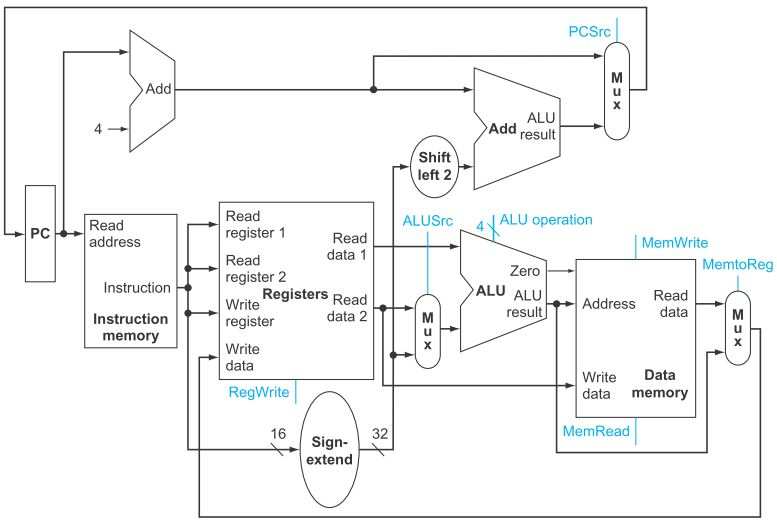
\includegraphics[scale=0.75]{Core datapath.JPG}
    \caption{The datapath for the memory instructions and the R-type instructions.}
\end{figure}
This datapath can execute the basic instructions e.g. load-store word, ALU operations, and branches
in a single clock cycle. Just one additional multiplexor is needed to integrate branches.

Given this simple datapath, a control unit is needed:
\begin{itemize}
    \item Take inputs and generate a write signal for each state element.
    \item Acts as the selector control for each multiplexor.
    \item Control the \texttt{ALU}.
\end{itemize} 

\pagebreak
%%%%%%%%%%%%%%%%%%%%%%%%%%%%%%%%%%%%%%%%%%%%%%%%%%%%%%%%%%%%%%%%%%%%%%%%%%%%%%%%%%%%%%%%%%%%%%%%%%%%%%%%%%
\section{A Simple Implementation Scheme}

Implementation of a MIPS subset includes designing \textbf{a data path} and \textbf{the suitable control
functions}. 

This simple implementation uses the datapath of the last section and a simple control function. It
supports \texttt{lw}, \texttt{sw}, \texttt{beq}, and arithmetic-logical instructions \texttt{add},
\texttt{sub}, \texttt{AND}, \texttt{OR}, and \texttt{set on less than}. 

\begin{figure} [h!]
    \centering
    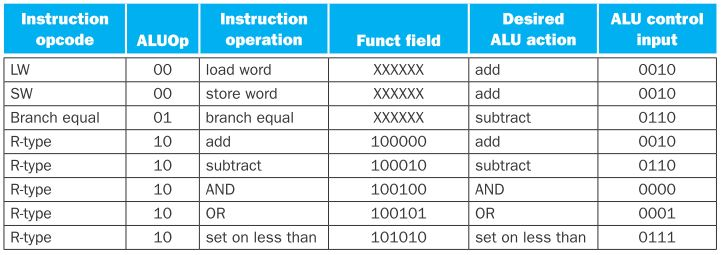
\includegraphics[scale=0.8]{ALU instructions.JPG}
    \caption{How ALU control bits are set depending on the \texttt{ALUOp} control bits and the different function field for the R-type instruction.}
\end{figure}
%%%%%%%%%%%%%%%%%%%%%%%%%%%%%%%%%%%%%%%%%%%%%%%%%%%%%%%%%%%%%%%%%%%%%%%%%%%%%%%%%%%%%%%%%%%%%%%%%%%%%%%%%%
\subsection{ALU control}

In MIPS, depending on the instruction class, the ALU will need to perform one of six functions.
\begin{figure} [h!]
    \centering
    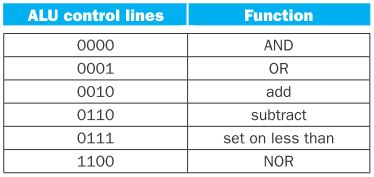
\includegraphics[scale=0.7]{ALU basic.JPG}
\end{figure}

For example:
\begin{itemize}
    \item \texttt{lw} and \texttt{sw} instructions, the ALU computes the memory address by addition
    \item R-type instructions, ALU needs to perform one of the five actions (AND, OR, subtract, 
    add, or set on less than) depending on the value of the 6-bit \texttt{funct field}
\end{itemize}  

\pagebreak

The \textbf{4-bit ALU control input} is set using a control unit with two inputs:
\begin{itemize}
    \item The function field of the instruction
    \item \texttt{ALUOp}: A $2$-bit control field indicating whether the operation to be performed should be:
    \begin{itemize}
        \item $00$: Loads and Stores
        \item $01$: Subtract for \texttt{beq}
        \item $10$: Determined by the operation encoded in the \texttt{funct field}
        
        Note: The function field \textbf{is only used} when the \texttt{ALUOp} bits equal 10, a small piece
        of logic that recognizes the subset of possible values is used.
    \end{itemize}
\end{itemize} 

\begin{figure} [h!]
    \centering
    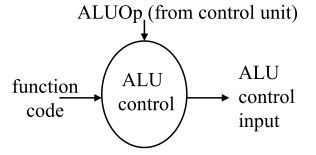
\includegraphics[scale=0.7]{ALU diagram.JPG}
\end{figure}

The output of the \texttt{ALU control unit} is a 4-bit signal directly controlling the \texttt{ALU}
by generating one of the 4-bit combinations shown above.

This design uses multiple levels of decoding i.e. the \texttt{main control unit} generates the
\texttt{ALUOp} bits, which then are used as input to the \texttt{ALU control unit} that generates the actual
signals to control the \texttt{ALU}. This is a common implementation technique because using multiple levels of control can:
\begin{itemize}
    \item Reduce the size of the main control unit
    \item Potentially increase the speed of the control unit
\end{itemize} 
These optimizations are important because the speed of the control unit is critical to the clock cycle time.

\pagebreak
%%%%%%%%%%%%%%%%%%%%%%%%%%%%%%%%%%%%%%%%%%%%%%%%%%%%%%%%%%%%%%%%%%%%%%%%%%%%%%%%%%%%%%%%%%%%%%%%%%%%%%%%%%
\subsection{Designing the Main Control Unit}

Identify the fields of an instruction and the control lines that are needed for the datapath
constructed above: 
\begin{figure} [h!]
    \centering
    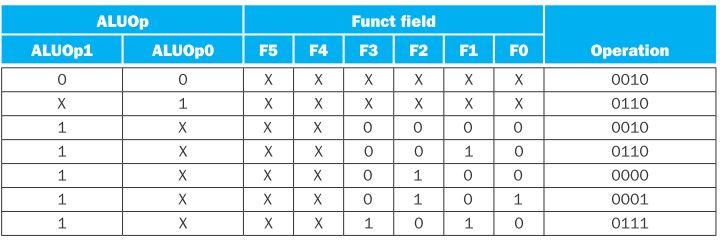
\includegraphics[scale=0.7]{ALU simplified.JPG}
    \caption{ The truth table for the 4 ALU control bits}
\end{figure} 

To see the relationship of the fields of an instruction and the datapath, view the formats of the
three instruction classes: the R-type, branch, and load-store.
\begin{figure} [h!]
    \centering
    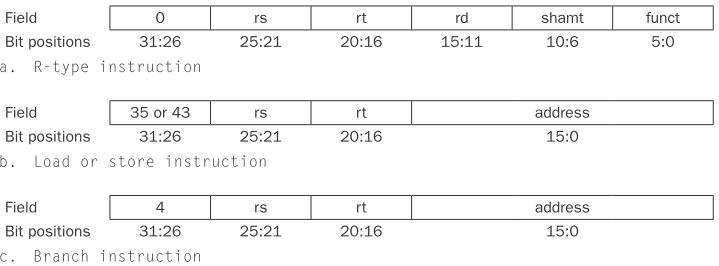
\includegraphics[scale=0.75]{Three types.JPG}
\end{figure} 

\begin{tcolorbox}[breakable,colback=white]
\textbf{Opcode}: The field that denotes the operation and format of an instruction.
\end{tcolorbox}

Note: The design principle \textit{simplicity favors regularity} is seen here in specifying control.
There are several major observations about these instruction formats:
\begin{itemize}
    \item The \texttt{opcode} i.e. \textbf{Op[5:0]} is always contained in bits $[31:26]$.
    \item The two registers to be read are always specified by the \texttt{rs} at $[25:21]$ and
    \texttt{rt} at $[20:16]$. 
    \item The 16-bit off set for branch equal, load, and store is always in positions $[15:0]$.
    \item The destination register is in one of two places:
    \begin{itemize}
        \item For load it is in bit positions $[20:16]$
        \item For R-type instruction it is in bit positions $[15:11]$
    \end{itemize}

    Thus, a multiplexor is needed to select which field of the instruction is used to decide between
    the two positions.
\end{itemize}

Using these information, the instruction labels and extra multiplexor is added to the simple datapath. 
\begin{figure} [h!]
    \centering
    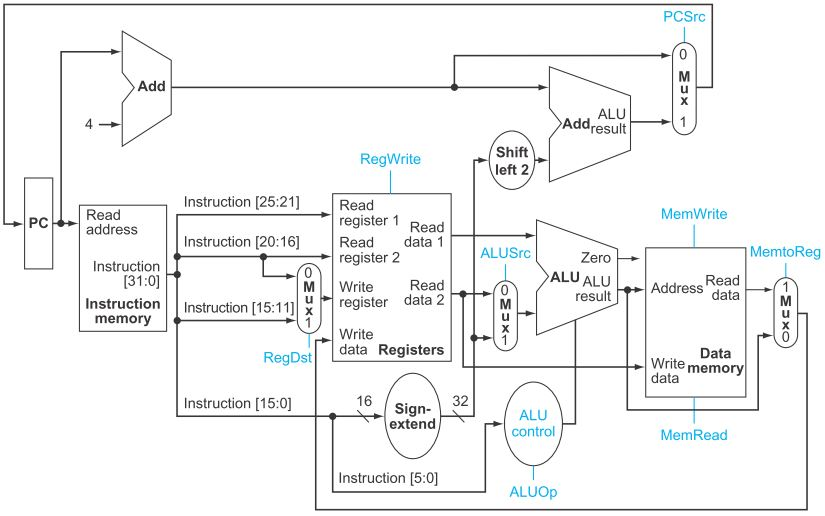
\includegraphics[scale=0.8]{Data path 2.JPG}
    \caption{Datapath with all necessary multiplexors and all control lines.}
\end{figure}

\begin{figure} [h!]
    \centering
    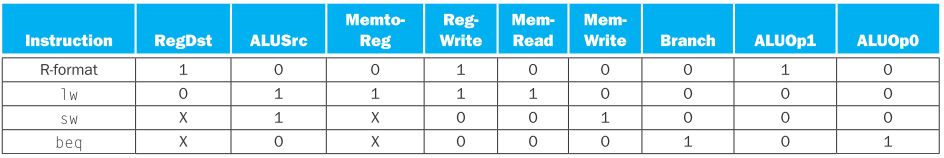
\includegraphics[scale=0.7]{R type control.JPG}
    \caption{The control lines determined by the \textit{OpCode} fields of the instruction.}
\end{figure}

\pagebreak

Next are the \textbf{seven single-bit control lines plus the 2-bit ALUOp control 
signal} where the \texttt{ALUOp control signal} is used to define what the seven other control
signals do. \par
\begin{figure} [h!]
    \centering
    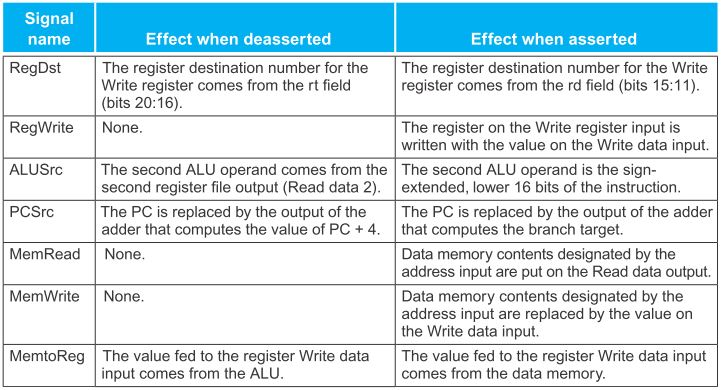
\includegraphics[scale=0.8]{Control signals.JPG}
    \caption{The effect of each of the seven control signals.}
\end{figure}
These nine control signals (seven from above and two for ALUOp) is determined by the six input
signals to the control unit i.e. the \texttt{Opcode} bits $[31:26]$. 

\begin{figure} [h!]
    \centering
    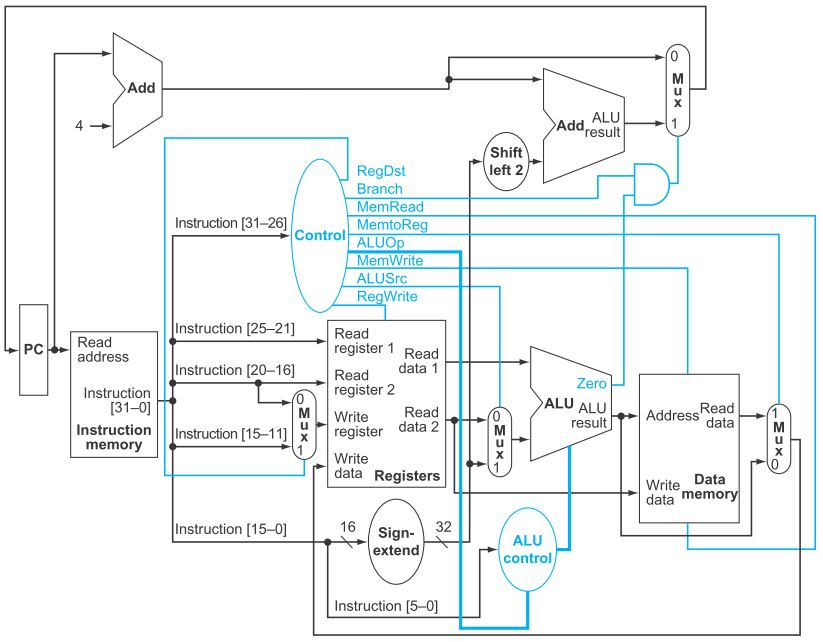
\includegraphics[scale=0.69]{MIPS with control.JPG}
    \caption{The simple datapath with the control unit}
\end{figure}

\pagebreak

%%%%%%%%%%%%%%%%%%%%%%%%%%%%%%%%%%%%%%%%%%%%%%%%%%%%%%%%%%%%%%%%%%%%%%%%%%%%%%%%%%%%%%%%%%%%%%%%%%%%%%%%%%
\subsection{Operation of the data path}

Based on the previous chapters, the information can be used to design the \textbf{control unit
logic}. To give a short summary, viewing how the three different instruction classes uses the datapath. 

The operation of the datapath for an \textbf{R-type instruction} e.g. \texttt{add \$t1,\$t2,\$t3}.
Everything occurs in \textbf{one clock cycle} and consists of the four steps that are ordered by the flow 
of information:
\begin{enumerate}
    \item An instruction is fetched from \textit{Memory} and the \textit{PC} is incremented.
    \item  
    \begin{itemize}
        \item Two registers \texttt{\$t2} and \texttt{\$t3} are read from the \textit{Register File}.
        \item The main control unit \textbf{computes and sets} the control lines.
    \end{itemize} 
    \item  \textit{ALU} processes the data read from the \textit{Register File} using the function 
    code i.e. instruction funct field $[5:0]$ from the \textit{ALU Control} to output the
    \textit{ALU} control code.
    \item Result from the \textit{ALU} is written into the \textit{Register File} using instruction bits $[15:11]$ to select the destination register \texttt{\$t1}.
\end{enumerate}

\begin{figure} [h!]
    \centering
    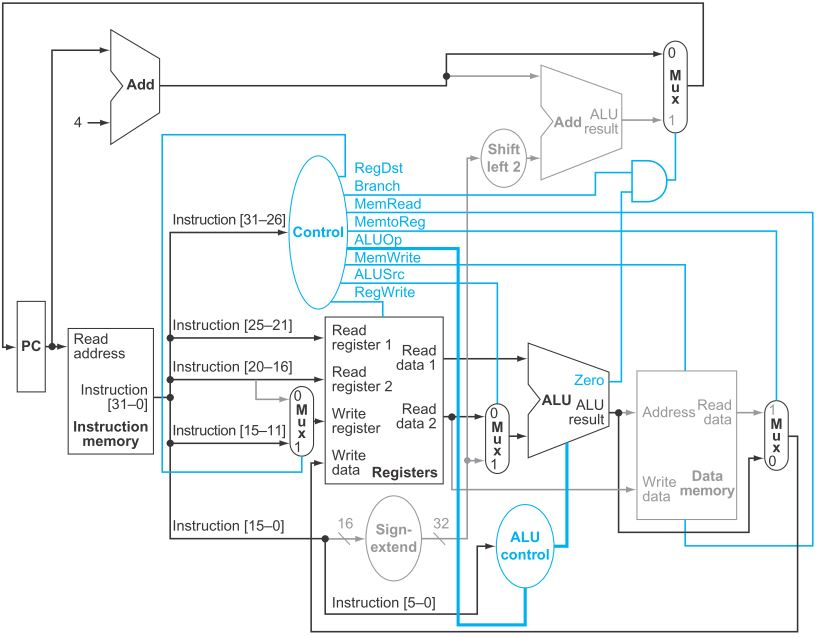
\includegraphics[scale=0.7]{Add.JPG}
    \caption{The datapath in operation for an R-type instruction, such as \texttt{add \$t1,\$t2,\$t3}.}
\end{figure}

\pagebreak

The execution of a load word instruction e.g. \texttt{lw \$t1, offset(\$t2)} can be shown in 5 steps:
\begin{enumerate}
    \item An instruction is fetched from \textit{Memory} and the \textit{PC} is incremented.
    \item Register \texttt{\$t2} value is read from the \textit{Register File}.
    \item \textit{ALU} computes the sum of the value read from: \textit{Register File} and the 
    \textbf{sign-extended, lower 16 bits, offseted instruction}.
    \item The sum from the \textit{ALU} is used as the address for the \textit{Data Memory}.
    \item 
    \begin{itemize}
        \item Data from \textit{Memory} is written into the \textit{Register File}.
        \item The register destination is given by instruction bits $[20:16]$ in register \texttt{\$t1}.
    \end{itemize} 
\end{enumerate}
\begin{figure} [h!]
    \centering
    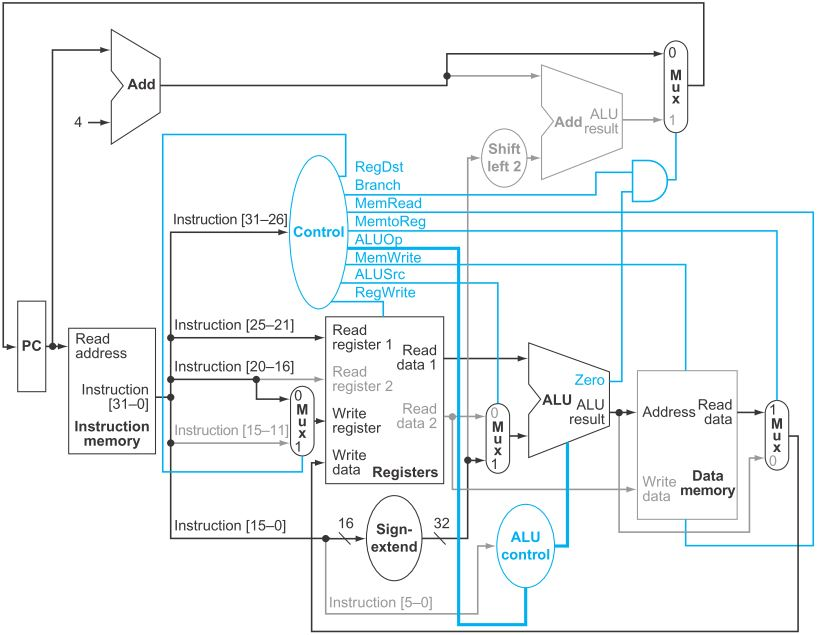
\includegraphics[scale=0.7]{lw.JPG}
    \caption{The datapath in operation for a load instruction.}
\end{figure}

\pagebreak

The execution of branch-on-equal instruction e.g. \texttt{beq \$t1, \$t2, offset}. It operates much
like an R-format instruction but the \textit{ALU} output is used to determine whether the
\textit{PC} is written with \textbf{PC + 4} or \textbf{branch target address}. It can be shown in
four steps:
\begin{enumerate}
    \item An instruction is fetched from \textit{Memory} and the \textit{PC} is incremented.
    \item Two registers \texttt{\$t2} and \texttt{\$t3} are read from the \textit{Register File}.
    \item 
    \begin{itemize}
        \item The \textit{ALU} perform subtraction \texttt{sub} on data values from the \textit{Register
        File}.
        \item The value \textbf{PC + 4} is added to the \textbf{sign-extended, lower 16 bits,
        offset left by 2 bits instruction}. 
        \item The result is the branch target address.
    \end{itemize} 
    \item The \textbf{Zero result} from the \textit{ALU} is used to decide which adder result to store 
    into the \textit{PC}.
\end{enumerate}
\begin{figure} [h!]
    \centering
    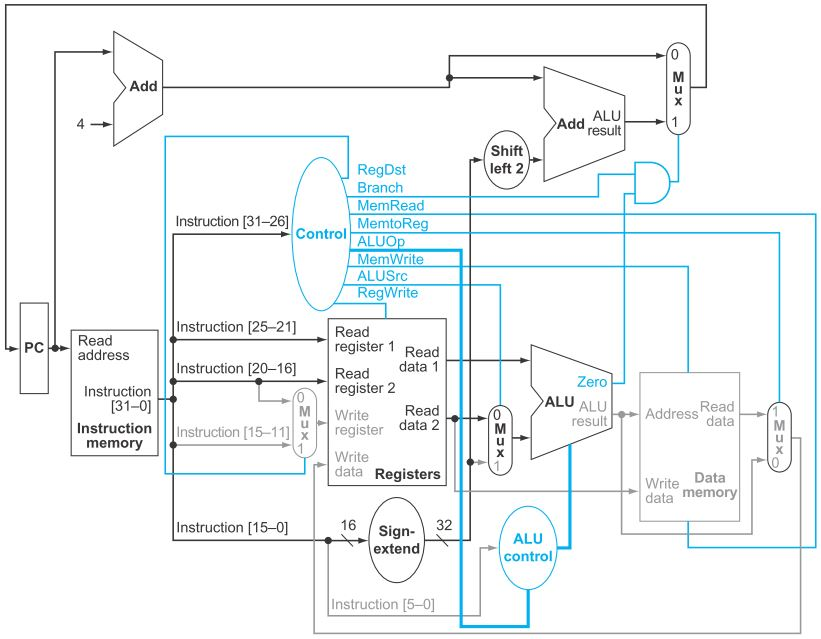
\includegraphics[scale=0.7]{beq.JPG}
    \caption{The datapath in operation for a branch-on-equal instruction. Note: After using the register file and ALU to perform the compare, the Zero output is used to select the next program 
    counter from between the two candidates.}
\end{figure}

\pagebreak

%%%%%%%%%%%%%%%%%%%%%%%%%%%%%%%%%%%%%%%%%%%%%%%%%%%%%%%%%%%%%%%%%%%%%%%%%%%%%%%%%%%%%%%%%%%%%%%%%%%%%%%%%%
\subsection{Finalising the Control}

The control function is defined using the contents of the following table: \par 
\begin{figure} [h!]
    \centering
    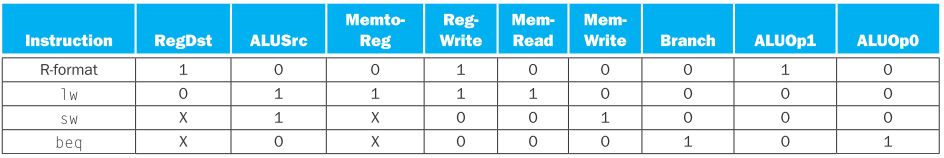
\includegraphics[scale=0.6]{R type control.JPG}
\end{figure}
\begin{itemize}
    \item \textbf{Input}: The $6$-bit \textit{OpCode} field: $\text{Op}[5:0]$
    \item \textbf{Outputs}: The control lines
\end{itemize}
A truth table for each of the outputs based on the binary encoding of the \textit{OpCodes} can be
produced:
\begin{figure} [h!]
    \centering
    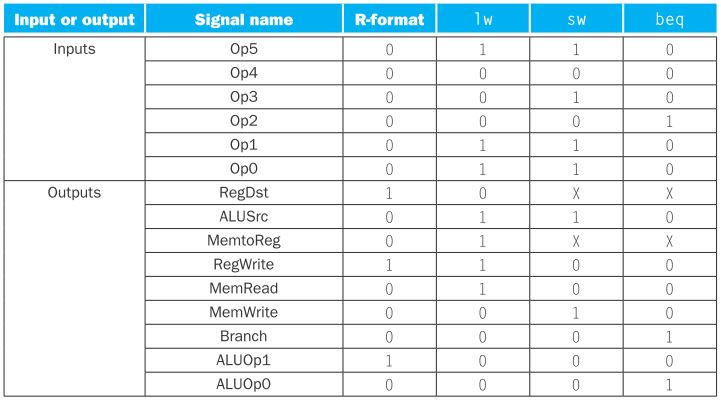
\includegraphics[scale=0.75]{Control table.JPG}
    \caption{The control function for the simple single-cycle implementation is completely specified by this truth table.}
\end{figure}

A \textbf{single-cycle implementation} of most of the MIPS core instruction set has been
implemented. 
\begin{tcolorbox}[breakable,colback=white]
\textbf{Single-cycle implementation} or \textbf{Single clock cycle implementation}: An
implementation in which an instruction is executed in one clock cycle. Easy to understand but too slow to be practical. 
\end{tcolorbox}

\pagebreak

%%%%%%%%%%%%%%%%%%%%%%%%%%%%%%%%%%%%%%%%%%%%%%%%%%%%%%%%%%%%%%%%%%%%%%%%%%%%%%%%%%%%%%%%%%%%%%%%%%%%%%%%%%
\subsection{Jump instructions}

The final step is to add jump instructions to the basic datapath and control unit. 

The jump instruction is similar to a branch instruction but has the following differences:
\begin{itemize}
    \item computes the target \textit{PC} differently
    \item is not conditional
\end{itemize}  

\begin{figure} [h!]
    \centering
    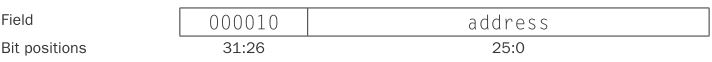
\includegraphics[scale=0.8]{Jump.JPG}
    \caption{Instruction format for the jump instruction (opcode = 2)}
\end{figure}

Calculating the $32$-bit binary jump address: 
\begin{itemize}
    \item Like branch instructions, the low-order (right) 2 bits of the binary jump address are $00$.
    \item The next lower $26$ bits of this $32$-bit address come from the 26-bit immediate field in the jump
    instruction.
    \item The upper $4$ bits of the address that should replace the \textit{PC} come from the \textit{PC} of the jump instruction plus 4.
\end{itemize}
This means a jump is implemented by storing into the \textit{PC} the concatenation of:
\begin{enumerate}
    \item  Upper $4$ bits of the current $PC + 4$ i.e. bits $[31:28]$ of the sequentially following instruction address.
    \item The $26$-bit immediate field of the jump instruction.
    \item The bits $00_{two}$
\end{enumerate}

To add the jump feature into the existing data path design, the following changes are made:
\begin{enumerate}
    \item An additional multiplexor used to select the source for the new \textit{PC} value which 
    is either:
    \begin{itemize}
        \item The incremented \textit{PC} i.e. $PC+4$
        \item The branch target \textit{PC} (Supports \texttt{beq})
        \item The jump target \textit{PC}
    \end{itemize} 
    \item One additional control signal required for the additional multiplexor called
    \textbf{Jump}. \textbf{Jump} is only asserted when instruction is a jump instruction i.e.
    \textit{OpCode} is 2
\end{enumerate}

\pagebreak
\begin{figure} [h!]
    \centering
    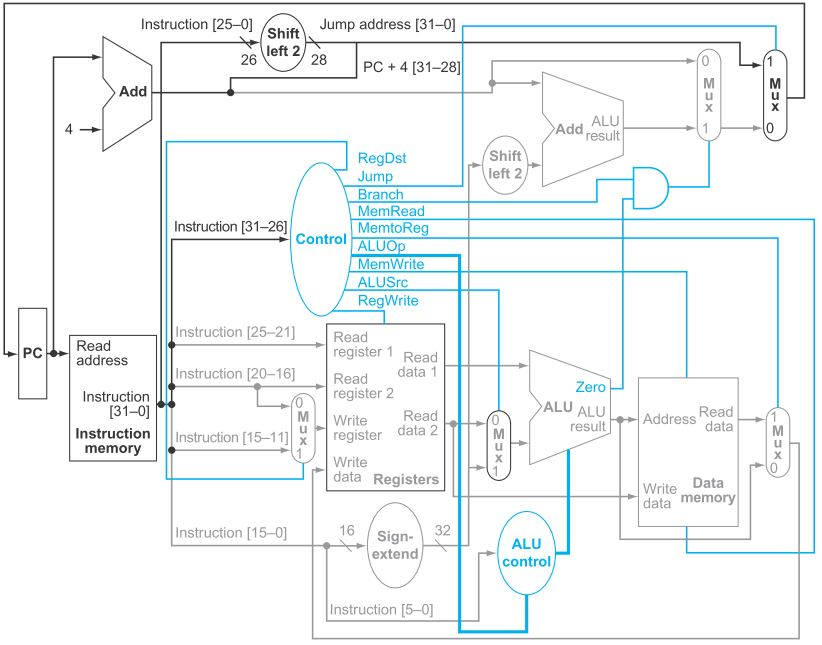
\includegraphics[scale=0.75]{Jump data path.JPG}
    \caption{The simple control and datapath are extended to handle the jump instruction}
\end{figure}

\pagebreak

%%%%%%%%%%%%%%%%%%%%%%%%%%%%%%%%%%%%%%%%%%%%%%%%%%%%%%%%%%%%%%%%%%%%%%%%%%%%%%%%%%%%%%%%%%%%%%%%%%%%%%%%%%
\section{Single-cycle implementation}

Single-cycle designs are not used in modern designs because it is inefficient.

Notice that the clock cycle must have the \textbf{same length for every instruction} in this
single-cycle design. Of course, \textbf{the longest possible path in the processor determines the clock
cycle}. In the MIPS instruction set, this path is a load instruction - five functional units are
used in series: 
\begin{itemize}
    \item the Instruction Memory
    \item the Register File
    \item the ALU
    \item the Data Memory
    \item the Register File
\end{itemize}

The penalty for using the single-cycle design with a fixed clock cycle is significant but it is acceptable for small instruction sets.


%%%%%%%%%%%%%%%%%%%%%%%%%%%%%%%%%%%%%%%%%%%%%%%%%%%%%%%%%%%%%%%%%%%%%%%%%%%%%%%%%%%%%%%%%%%%%%%%%%%%%%%%%%
\end{document}